\documentclass[12pt, twoside]{article}
\usepackage[letterpaper, margin=1in, headsep=0.5in]{geometry}
\usepackage[english]{babel}
\usepackage[utf8]{inputenc}
\usepackage{amsmath}
\usepackage{amsfonts}
\usepackage{amssymb}
\usepackage{tikz}
\usepackage{yhmath}
%\usetikzlibrary{quotes, angles}

\usepackage{graphicx}
\usepackage{enumitem}
\usepackage{multicol}

\usepackage{fancyhdr}
\pagestyle{fancy}
\fancyhf{}
\renewcommand{\headrulewidth}{0pt} % disable the underline of the header

\fancyhead[RE]{\thepage}
\fancyhead[RO]{\thepage \\ Name: \hspace{3cm}}
\fancyhead[L]{BECA / Dr. Huson / 10th Grade Geometry\\* 12 February 2020}

\begin{document}
\subsubsection*{8.11 Classwork: Volume of water tanks}
 \begin{enumerate}

  \item Find the area of the shape shown below composed of a rectangle and circular ends. Leave your answer as an exact value in terms of $\pi$.
  \begin{flushright}
  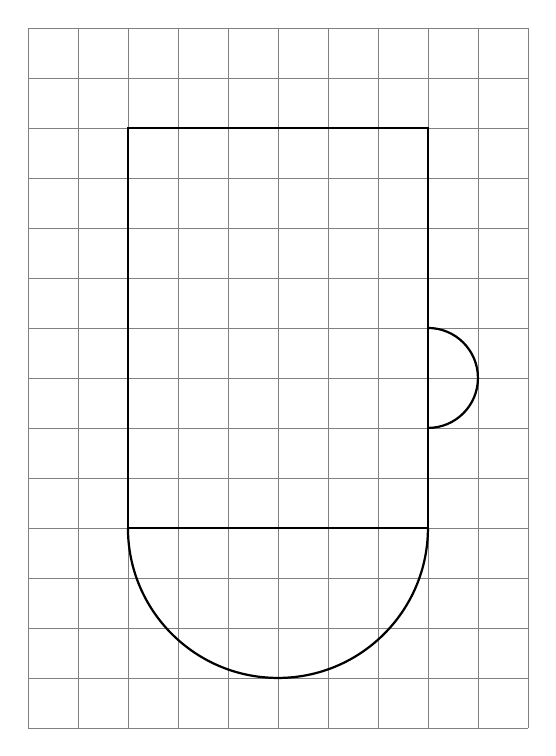
\begin{tikzpicture}[scale=.635]
    \draw [help lines] (-2,-4) grid (8,10);
    %\draw [thick, ->] (-2.2,0) -- (8.4,0) node [below right] {$x$};
    %\draw [thick, ->] (0,-1.2)--(0,7.4) node [left] {$y$};
    \draw [thick] (0,0)--(6,0)--(6,8)--(0,8)--cycle;
    \draw [thick] (0,0) arc (180:360:3);
    \draw [thick] (6,2) arc (-90:90:1);
  \end{tikzpicture}
\end{flushright}\vspace{1cm}

\end{enumerate}
\end{document}
